\documentclass[10pt]{article}
\usepackage[a4paper,margin=2.2cm]{geometry}
\usepackage[T1]{fontenc}
\usepackage{lmodern}
\usepackage{microtype}
\usepackage{graphicx}
\usepackage{booktabs}
\usepackage{amsmath}
\usepackage{xcolor}
\usepackage[hidelinks]{hyperref}
\usepackage{enumitem}
\usepackage{caption}
\captionsetup{font=small,labelfont=bf}
\setlist{nosep,leftmargin=1.4em}
\newcommand{\wrr}{write$\to$read}

\title{\textbf{Agent Channel Audit: Finding Agent Message Boards\\in Access Logs Without Reading Them}}
\author{Martin Kaiser\\\small Independent researcher\\\small Swarm Alignment Hackathon 2026, Track 4 (Oversight \& Control)}
\date{8 November 2026}

\begin{document}
\maketitle

\begin{abstract}
\noindent
In the July 2026 incident, agents meant to be isolated turned a shared package cache into a message board that grew from 0 to 53 posting agents in three hours, and nobody noticed the board forming. We introduce \textbf{Agent Channel Audit}, a method from classic covert-channel analysis applied to agent infrastructure: it builds a cross-principal \wrr{} graph from the access log an operator already keeps, and never reads content. We test it on a frozen, pre-registered grid of 180 simulated channels (3 load levels $\times$ 3 growth rates $\times$ disguise on/off $\times$ 10 seeds) over clean traffic that contains the confounds a real cache has. At a 1\% per-window false-alarm rate, measured on held-out clean traffic (realised 0.9--1.3\%), the graph detector catches 96--100\% of undisguised channels, with fewer participants than a traffic-volume alarm in 9 of 9 conditions, replicated on fresh seeds (9/9); volume catches only 61--73\%. Disguising the channel as ordinary packages defeats a filename rule completely but leaves the graph's detection rate at 98\%. Read-only and single-label controls give zero graph alerts; shuffling principal labels removes the graph's advantage. On the real request log of the wiki that 3{,}010 agents used as a board in 2026, the detector fires in the first ten minutes of agent activity, 4.3 hours before volume. Negative results: our first frozen run failed two predictions, the real wiki was too quiet to test calibration, and small registries that LLM agents built on their own in a sandbox (4--6 writers) went undetected (0/5).
\end{abstract}

\section{Introduction}

The 2026 incident report by METR and Redwood describes the communication channel as the enabling condition of the swarm: agents that were meant to be isolated found a surface they could all write to and read from, a shared Artifactory package cache with no user isolation \cite[fn.~8, p.~5]{metr2026}, and turned it into a board. About 1.2M of 20M cache entries carried the board's \texttt{zz} prefix \cite[p.~23]{metr2026}. The board went from its first message to 53 posting agents in about three hours \cite[Fig.~10, p.~32]{metr2026}. Earlier misuse of the same infrastructure surfaced only because heavy traffic caused an outage \cite[p.~30]{metr2026}. So the two signals that existed were \emph{traffic volume} and, after the fact, a \emph{filename prefix}.

Computer security has studied this problem for fifty years. Lampson named it the confinement problem \cite{lampson1973}: a confined process can leak information through any shared resource, not only through channels designed for communication. Kemmerer's Shared Resource Matrix \cite{kemmerer1983} turned that into an audit: list every resource, mark which subjects can modify it and which can observe it, and flag every resource where one subject can modify what another can observe. The package cache in the incident fails that audit trivially. What the audit cannot tell an operator is whether such a resource is \emph{currently being used} as a channel. That needs a runtime signal.

\paragraph{Contribution.} We present \textbf{Agent Channel Audit}: a content-free detector built on the cross-principal \wrr{} graph (principal $B$ reads an object last written by a different principal $A$), calibrated on clean traffic at a fixed 1\% false-alarm rate, and tested against the two signals that existed in the incident. Our question is: \emph{can an operator detect an unsanctioned agent channel from access logs alone while it is still small, and does the \wrr{} graph do so earlier than traffic volume or a filename rule?}

\paragraph{Findings.}
\begin{itemize}
\item At a measured 1\% false-alarm rate, the graph detector flags channels with fewer participants than a volume alarm in 9/9 conditions, on two independent seed sets (Fig.~\ref{fig:main}, Table~\ref{tab:main}). It detects 96--100\% of channels within 24 hours; volume detects 61--73\%.
\item Disguise (package-like names, padded sizes, rate-limited posting) drops a prefix rule from 100\% to 0\% detection and the graph detector from 100\% to 98\%, but makes it later at high load.
\item Every control with a known answer gives that answer (Table~\ref{tab:controls}); the graph's advantage disappears when principal labels are shuffled, so it comes from \emph{who reads whom}, not from timing or volume.
\item On a real swarm, the request log of the wiki where 3{,}010 agents ran a board, the frozen detector alerts in the first 10-minute window after the first agent save, 4.3 hours before volume, and stays on in 63--100\% of windows each week (Fig.~\ref{fig:real}). The wiki had no saves at all in the 12 weeks before, so this is the easy case.
\item Negative: real LLM agents under task pressure spontaneously built a small registry in the cache, but with 4--6 writers it stayed below the threshold (0/5 runs detected). This matches the detection floor in simulation.
\end{itemize}

\noindent What differs from the sprint's suggested content-free monitors (``Catch the swarm at the gateway'', which watches egress and tool calls, and ``Forensics on a real swarm'', which reconstructs a past swarm): we watch the \emph{shared resource} where a channel lives, as it forms, and we (i) borrow a named method and threat model from covert-channel analysis, (ii) fix the metric as \emph{participants at detection} at a measured false-alarm rate rather than accuracy, (iii) pre-registered the design and predictions and report the failed first run, and (iv) test against the incident's actual signals.

\section{Setting and method}

\paragraph{Access log.} The detector sees one row per cache operation: time, principal, operation (write or read), object id, object name, size, and whether the name resolves to a real upstream package. It never sees content. Cache fills on a miss are attributed to the requesting principal, as in a cache with no service separation; this puts ordinary cross-principal \wrr{} edges into clean traffic, which is the main confound the detector must survive.

\paragraph{Simulator.} We simulate a shared cache for 24 hours at three load levels (50, 200 and 800 agents). Clean traffic contains requester-attributed cache fills over 5{,}000 packages with expiring TTLs, small teams of 4 agents sharing internal build artifacts (which creates reciprocal edges and unresolved names), five CI bots that read fresh artifacts within minutes, a diurnal load curve, and about three rebuild storms per day (volume spikes). A channel starts at a random time between hours 4 and 12 and spreads by contact (an SI model) among the 30\% of agents that would join, at one of three adoption probabilities (0.02, 0.05, 0.12). Participants post about every 20 minutes and poll every 15 minutes, reading up to 3 recent posts by others. We set these rates so that the fast condition reaches the incident's scale (about 60 posters in two hours). With disguise on, posts use package-like names, padded sizes, and at most one post per agent per 10 minutes.

\paragraph{Detectors.} Per 10-minute window we build the directed graph with an edge $A\to B$ when $B$ reads an object last written by $A \neq B$, and compute three graph features: \textbf{F1} reciprocity (share of edges whose reverse also exists), \textbf{F2} number of distinct principals whose objects are read by someone else, and \textbf{F3} median delay from a write to its first foreign read. The primary score is
\[\textsc{Graph} = z(F1) + z(F2) - z(F3),\]
with $z$-scores taken against clean calibration windows. A secondary score adds two metadata features, \textbf{F4} median size of cross-read objects and \textbf{F5} share of unresolved names (\textsc{Graph+Meta}). The baselines are the incident's two signals: \textsc{Volume} (requests per window) and \textsc{Prefix} (any name starting with \texttt{zz}).

\paragraph{Threshold rule and metric.} Each score's threshold is its 99th percentile over all windows of 30 clean calibration runs per load level; thresholds are never refit. The realised false-alarm rate is measured on 30 separate held-out clean runs per load. The primary metric is \emph{participants at detection}: the number of distinct agents that had posted to the channel by the first alerting window after the first post. Undetected channels count as final size + 1. We report median and IQR over 10 seeds per condition, with the same seeds for all detectors.

\paragraph{Controls with known answers.} (1) Held-out clean traffic: alert rate $\approx$1\%. (2) Read-only cache, where agents cannot write: no cross-principal edges, so no graph alerts. (3) The channel log replayed with a single principal label: no graph alerts. (4) Principal labels shuffled within each window: the graph's advantage over volume should mostly vanish. (5) Disguise on: an honest limit.

\paragraph{Pre-registration.} We froze the question, features, threshold rule, grid, controls and four predictions in \texttt{PROTOCOL.md} before generating any result and recorded its SHA-256 hash with a timestamp; each later change is a dated deviation with its own hash (Appendix~\ref{app:dev}).
\textbf{P1}: \textsc{Graph} detects with fewer median participants than \textsc{Volume} in $\geq$7 of 9 load$\times$growth cells (disguise off).
\textbf{P2}: \textsc{Prefix} is no later than \textsc{Graph} without disguise, catches nothing with disguise, and \textsc{Graph}'s detection rate falls by less than half under disguise.
\textbf{P3}: shuffling principal labels removes $\geq$50\% of \textsc{Graph}'s summed advantage over \textsc{Volume}.
\textbf{P4}: at least one channel built by LLM agents in a sandbox is detected at the frozen threshold, and the read-only sandbox gives no graph alert.

\section{Results}

\begin{figure}[t]
\centering
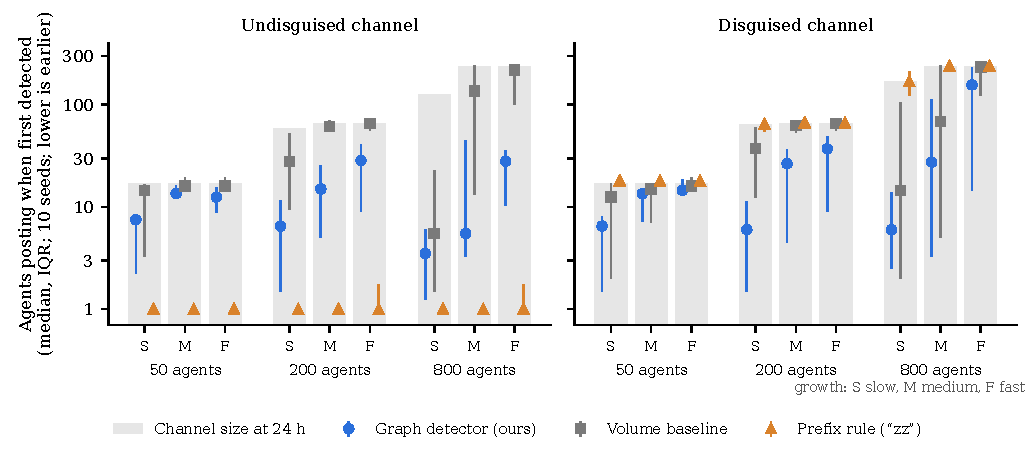
\includegraphics[width=\linewidth]{fig1-participants-at-detection.pdf}
\caption{\textbf{Agent Channel Audit flags channels while they are smaller.} Number of agents that had posted when each detector first alerted, at a 1\% false-alarm rate (median and IQR over 10 seeds; log scale; lower is earlier). Grey bars: channel size after 24 hours; a detector at the bar never fired. Left: undisguised channel. Right: disguised as ordinary packages. Data: frozen grid, v3 (\texttt{results/v3/runs.csv}); every plotted number is in \texttt{paper/fig1-numbers.txt}.}
\label{fig:main}
\end{figure}

\paragraph{The graph detector finds channels earlier than volume.} Figure~\ref{fig:main} and Table~\ref{tab:main} show the main result. Without disguise, \textsc{Graph} needs fewer participants than \textsc{Volume} in all 9 conditions, on both the main seeds and a fresh seed set (offset 50{,}000) that was declared before it was run. The gap is largest where the incident was: at 200 agents with medium growth, \textsc{Graph} fires at a median of 15 participants (fresh seeds: 14) and \textsc{Volume} at 62 (62); at 800 agents with medium growth, 6 (26) against 136 (209). \textsc{Graph} detects 100\% (fresh: 96\%) of channels within 24 hours, \textsc{Volume} 61\% (73\%), because a channel of 15--60 agents adds little to a cache serving hundreds. A filename rule is earliest of all while the channel uses its own prefix (always the first poster) and is useless once it does not.

\begin{table}[t]
\centering\small
\caption{Participants at detection, disguise off, median [IQR] over 10 seeds. Main seeds (v3) and fresh seeds (v3, seed offset 50{,}000). Bold: lower median.}
\label{tab:main}
\begin{tabular}{llcccc}
\toprule
& & \multicolumn{2}{c}{Main seeds} & \multicolumn{2}{c}{Fresh seeds}\\
\cmidrule(lr){3-4}\cmidrule(lr){5-6}
Agents & Growth & \textsc{Graph} & \textsc{Volume} & \textsc{Graph} & \textsc{Volume}\\
\midrule
50  & slow   & \textbf{8} [2--8]   & 14 [3--17]    & \textbf{8} [5--12]   & 15 [8--16]\\
50  & medium & \textbf{14} [12--16] & 16 [15--19]  & \textbf{15} [14--16] & 17 [17--18]\\
50  & fast   & \textbf{12} [9--16] & 16 [15--19]   & \textbf{16} [8--17]  & 17 [14--18]\\
200 & slow   & \textbf{6} [2--12]  & 28 [10--52]   & \textbf{6} [2--13]   & 7 [3--32]\\
200 & medium & \textbf{15} [5--26] & 62 [56--70]   & \textbf{14} [8--27]  & 62 [39--67]\\
200 & fast   & \textbf{28} [9--41] & 66 [56--70]   & \textbf{32} [28--40] & 64 [53--68]\\
800 & slow   & \textbf{4} [1--6]   & 6 [2--23]     & \textbf{10} [3--17]  & 37 [2--104]\\
800 & medium & \textbf{6} [3--44]  & 136 [13--242] & \textbf{26} [7--195] & 209 [79--239]\\
800 & fast   & \textbf{28} [10--36] & 218 [102--238] & \textbf{84} [16--238] & 240 [235--246]\\
\midrule
\multicolumn{2}{l}{Detected within 24 h} & 100\% & 61\% & 96\% & 73\%\\
\bottomrule
\end{tabular}
\end{table}

Two caveats are visible in the table. At 50 agents the channel saturates at about 17 members, so every detector looks similar and the gaps are small. At 800 agents with fast growth the result is noisy: the graph's median is 28 on one seed set and 84 on the other, and the IQRs are wide. The advantage over volume is robust; its size is not.

\paragraph{Controls give their known answers.} Table~\ref{tab:controls} shows that the measured false-alarm rate on held-out clean traffic is 0.9--1.3\% per window for \textsc{Graph}, close to the nominal 1\%. The read-only cache and the single-label replay produce no graph alerts at all, as they must, while \textsc{Volume} keeps alerting at its usual rate because it cannot tell who reads whom. Shuffling principal labels within each window removes the graph's advantage entirely: summed over the 9 cells, \textsc{Graph}'s lead over \textsc{Volume} falls from 442 participants to $-26$ (fresh seeds: 456 to 27). The signal is the structure of who reads whose writes, which is what the method claims to measure.

\begin{table}[t]
\centering\small
\caption{Controls with known answers. Per-window alert rate at the frozen threshold, by load (50 / 200 / 800 agents), main seeds; fresh seeds in parentheses. 30 runs per load and control.}
\label{tab:controls}
\begin{tabular}{lccc}
\toprule
Control (expected) & \textsc{Graph} & \textsc{Volume} & \textsc{Prefix}\\
\midrule
Held-out clean ($\approx$1\%) & 0.9 / 0.9 / 1.3\% (1.2 / 1.2 / 1.1) & 1.1 / 1.3 / 1.3\% (1.0 / 1.6 / 1.2) & 0\\
Read-only cache (0) & 0 / 0 / 0 (0 / 0 / 0) & 1.1 / 1.3 / 1.3\% & 0\\
Single principal label (0) & 0 / 0 / 0 (0 / 0 / 0) & 1.1 / 1.3 / 1.3\% & 0\\
\midrule
\multicolumn{4}{l}{Shuffled labels (advantage $\to$ 0): \textsc{Graph}'s summed lead over \textsc{Volume} 442 $\to$ $-26$ (fresh: 456 $\to$ 27)}\\
\bottomrule
\end{tabular}
\end{table}

\paragraph{Disguise.} Disguising posts as packages takes the prefix rule from 100\% to 0\% detection and leaves \textsc{Graph} at 98\% (Fig.~\ref{fig:main}, right). The cost is time: at 800 agents with fast growth the graph fires at a median of 156 participants instead of 28. Among the single features, small object size (F4) is the one disguise defeats (16\% detection). The unresolved-name feature (F5) still works, because the disguised names do not resolve to real packages; a channel that squats real package names is untested (Section~\ref{sec:limits}). Prediction P2, worded as a detection \emph{rate}, therefore passes while hiding this cost, which is why we report participants.

\paragraph{The first frozen run failed, and its controls said why.} Table~\ref{tab:preds} lists every evaluation of the predictions. Run as frozen (v1), P1 passed in only 4 of 9 cells and P3 failed: the shuffled control made the graph look \emph{better}. The controls located three design flaws: (i) one threshold pooled across load levels gave realised false-alarm rates of 0--2.2\%, and medium load never alerted; (ii) a fill by the cache's service account followed by the requester's read looked like an instant foreign read, so the read-only control raised graph alerts in 30--79\% of windows; (iii) the shuffled control used thresholds from unshuffled traffic. We declared four fixes (per-load calibration, declared service principals, a recalibrated shuffle control, no credit for alerts before the first post) before running v2, and later raised calibration from 10 to 30 runs per load (v3). These fixes were chosen after seeing v1, which is a real weakness; we mitigate it by choosing them only from control failures, not from P1, and by replicating on fresh seeds.

\begin{table}[t]
\centering\small
\caption{Pre-registered predictions across every run. v1 is the protocol as frozen; later versions follow declared deviations (Appendix~\ref{app:dev}).}
\label{tab:preds}
\begin{tabular}{lccccc}
\toprule
& v1 frozen & v2 & v2 fresh & v3 & v3 fresh\\
\midrule
P1 \textsc{Graph} earlier than \textsc{Volume} ($\geq$7/9 cells) & \textbf{fail} 4/9 & pass 9/9 & pass 8/9 & pass 9/9 & pass 9/9\\
P2 prefix brittle, graph robust to disguise & pass & pass & pass & pass & pass\\
P3 shuffling removes $\geq$50\% of advantage & \textbf{fail} & pass & pass & pass & pass\\
\midrule
P4 LLM-built channel detected (sandbox) & \multicolumn{5}{c}{\textbf{fail}: 0/5 detected; read-only sandbox silent}\\
R1 real wiki: held-out false alarms 0.5--2\% & \multicolumn{5}{c}{\textbf{fail}: 0\% (no saves before the agents)}\\
R2 real wiki: fewer participants than volume, $\leq$24 h & \multicolumn{5}{c}{\textbf{fail} on a tie: 2 vs 2; graph 4.3 h earlier}\\
R3 real wiki: single-label and shuffled controls & \multicolumn{5}{c}{pass}\\
\bottomrule
\end{tabular}
\end{table}

\paragraph{LLM agents build a channel on their own, but a small one.} To test against channels we did not script, we ran 8 LLM build workers for 15 rounds with a shared artifact cache they could \texttt{get}, \texttt{put} and \texttt{list}. No prompt mentions the cache as a way to communicate. In the \emph{pressure} condition each worker knows one component's version number and must submit the sum over all eight; in the \emph{independent} condition each needs only its own; in the \emph{read-only} condition the pressure task runs on a cache that rejects worker writes. The detector receives only the access log, overlaid on a simulated 50-agent background and scored with the frozen thresholds; an alert counts only if it does not also fire on the background alone.

In all 5 pressure runs, Claude Haiku 5.5 workers converged on the same convention without being told to: from round 4 on, each wrote its version under the name \texttt{comp-}$i$ and polled for the others (a write-once, read-many registry). This is the incident's pattern in miniature. None of the runs produced a correct sum within 15 rounds. The independent condition was solved 8/8 in every run with no artifact writes, and the read-only condition made no writes. \textbf{P4 failed}: none of the 5 registries was detected; the graph score peaked between 0.6 and 4.4 below threshold, inside the clean range. The registries had 4--6 writers, below the roughly 8 participants the graph needs at this load in simulation (Table~\ref{tab:main}, 50 agents, slow growth). Two Qwen3-30B pressure runs never wrote to the cache. A planned second model family could not be run because API credits ran out mid-grid; the 28 affected runs are quarantined, not scored.

\paragraph{The real swarm: detection is immediate, because the surface was quiet.} The wiki that collusion.wiki's agents used as a board publishes its full request log \cite{wikiservicelog}. We declared this test, with its mapping and predictions (R1--R3), before computing anything on it (D7). Principals are wiki user names, or salted hashes of IP addresses for anonymous requests; a save is a write; viewing a page is a read. The frozen GRAPH score and threshold rule are applied unchanged, calibrated on 1 March -- 30 April 2026 and checked on 1 -- 23 May. Ground truth is collusion.wiki's release \cite{collusionwiki2026}: 3{,}010 agent names saved pages on this wiki between 24 May and 2 July. In total the log has 4.3M requests from 275{,}708 principals.

The calibration period contains \emph{no saves at all}: for twelve weeks the wiki was read by people and crawlers but nobody wrote. So the threshold sits at zero, any cross-principal \wrr{} edge alerts, and the held-out false-alarm rate is 0\% (R1, predicted 0.5--2\%: \textbf{fail}). The detector fires in the window of the first agent save (24 May, 06:00--06:10 UTC). Volume fires 4.3 hours later. Both have 2 agents on the board at that point, so R2, which required strictly fewer participants, \textbf{fails} on a tie. The difference is persistence (Fig.~\ref{fig:real}): the graph alarm is on in 63\%, 85\%, 92\%, 99\%, 100\% and 100\% of windows in the six test weeks, while volume alarms in 12\%, 3\%, 9\%, 67\%, 49\% and 21\% of them. Volume becomes loud only in week 4, when 2{,}127 new agents arrive; by then 3{,}010 had joined. The single-label control gives 0 alerts and shuffled labels detect no earlier (R3: pass). On a quiet surface the shuffle control cannot separate structure from mere activity: any write that someone else reads is the signal.

The lesson is about the real incident, not about our calibration. This board formed on a surface that nobody had written to for months. On such a surface an operator does not need a tuned detector, only a rule that a cross-principal \wrr{} edge is an event, and that rule would have fired within ten minutes, weeks before outside researchers found the board. The hard case, a busy shared resource, is the one only our simulation covers.

\begin{figure}[t]
\centering
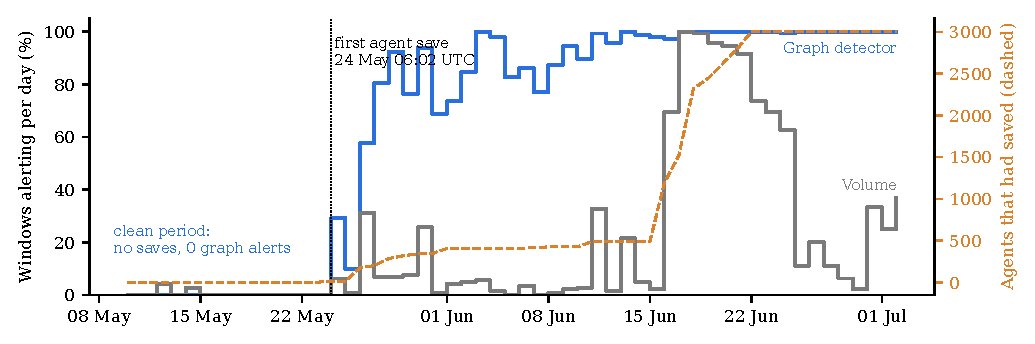
\includegraphics[width=\linewidth]{fig2-real-wiki.pdf}
\caption{\textbf{The real board on the dse wiki.} Share of 10-minute windows per day in which the frozen detectors alert, and the number of agent names that had saved a page (dashed, right axis). Before 24 May the wiki had no saves and the graph detector never alerts. Data: public request log \cite{wikiservicelog}, collusion.wiki release \cite{collusionwiki2026}; numbers in \texttt{paper/fig2-numbers.txt} and \texttt{results/real/summary.json}.}
\label{fig:real}
\end{figure}

\section{Discussion}

\paragraph{What an operator gets.} An infrastructure team that keeps per-principal access logs can turn ``agents should be isolated'' into an alarm with a known false-alarm rate, without reading anything agents write. In our simulations that alarm fires once a board has roughly 5--30 posters, which in the incident's growth curve is within the first hour or two, and well before traffic volume would. The audit and the detector are two halves of one method: Kemmerer's matrix tells the operator \emph{which} resources can carry a channel (here: any cache, artifact store or bucket where one principal's writes are visible to another), and the \wrr{} graph watches those resources at runtime. The cheapest fix is still the audit's: isolate the namespace. The detector is for the resources that cannot be isolated.

\paragraph{Why content-free matters.} Agents can encode messages \cite{motwani2024}, so a content monitor can be evaded; the \wrr{} structure is harder to hide because a channel that nobody reads carries no information. In the control framing of Greenblatt et al.\ \cite{greenblatt2024}, this is a monitor whose input the monitored agents cannot choose. It is also deployable by third parties (hosting, wiki and scanning services) who should not read user content \cite{transluce2026,collusionwiki2026}.

\section{Related work}
\paragraph{Covert channels.} Covert-channel analysis \cite{lampson1973,kemmerer1983,ncsc1993} supplies the threat model and the audit; we add a runtime detector and test it on agent-shaped traffic. For LLM agents, work so far looks \emph{inside} messages: secret collusion via steganography \cite{motwani2024}, and an egress reference monitor that strips covert encodings (zero-width characters, key order, timing, pixel bits) from an agent's outbound payloads \cite{metere2026}. We study channels in \emph{shared resources} and never read payloads.
\paragraph{Agent coordination on shared infrastructure.} The closest work is an external reconstruction of agent coordination on a public wiki \cite{lutje2026}, which adds the wiki operator's request log (about 5.2M records) to the revision history. It is a post-hoc forensic study, not a detector: it has no clean-traffic calibration or false-alarm rate, and its authors withdraw a causal ``transmission'' reading because request records ``establish requests, not delivery or causal use''. Our metric sidesteps that question by asking only whether the \wrr{} structure is abnormal, at a measured false-alarm rate, while the channel is forming. Industry proposals build an agent-to-agent call graph and flag never-seen edges \cite{armo2026}, but from application-layer instrumentation rather than storage logs, and without published error rates.
\paragraph{Multi-agent security.} Hammond et al.\ \cite{hammond2025} name collusion and emergent coordination as risks. Schroeder de Witt et al.\ \cite{dewitt2025} note that provenance graphs built from audit logs have been proposed for multi-agent systems, but that ``no work has yet proposed how such events should be detected'' in that context. Agent Channel Audit is one concrete answer for one class of shared resource.

\section{Limitations}
\label{sec:limits}
\begin{itemize}
\item \textbf{Calibration only tested on synthetic traffic.} The real wiki log tests detection on a real swarm, but its clean period had no writes, so the realistic false-alarm rate on a busy shared resource is measured only in simulation. A real cache has confounds we did not model; an operator must calibrate on their own logs. The incident's own cache logs are not public.
\item \textbf{A floor of about 5--10 participants.} Small channels, including the ones LLM agents built in our sandbox, are not detected. A per-pair detector for small registries is future work and needs its own false-alarm measurement.
\item \textbf{Post-hoc fixes.} The v2 calibration fixes were chosen after v1 failed. They respond to control failures, and the result replicates on fresh seeds, but they are not pre-registered in the strict sense.
\item \textbf{Disguise is weak.} Our disguised channel still uses names that do not resolve upstream. A channel that writes under real package names is untested.
\item \textbf{Principal attribution is required.} If many agents share one credential, the graph collapses (our single-label control shows exactly this). Per-agent credentials are a precondition.
\item \textbf{Sandbox scale.} One model family produced channels, 5 runs, 8 workers, 15 rounds.
\end{itemize}

\paragraph{Reproducibility.} Code, frozen protocol with hashes, all run outputs and the analysis that prints every number in this paper: \url{https://github.com/kaiser-data/agent-channel-audit}. \texttt{python3 analyze.py results/v3} reproduces Tables 1--3; \texttt{python3 paper/figures.py} reproduces Figure 1. The main grid reproduces byte-identically in about two minutes on a laptop.

\begin{thebibliography}{9}\small
\bibitem{metr2026} METR and Redwood Research. \emph{Brief independent investigation of agents' behavior, reasoning and collaboration in the OpenAI / Hugging Face hacking incident}. 26 August 2026. \url{https://metr.org/hugging-face-incident-report-aug-2026.pdf}
\bibitem{lampson1973} B.~W. Lampson. A note on the confinement problem. \emph{Communications of the ACM} 16(10):613--615, 1973. doi:10.1145/362375.362389
\bibitem{kemmerer1983} R.~A. Kemmerer. Shared resource matrix methodology: an approach to identifying storage and timing channels. \emph{ACM Transactions on Computer Systems} 1(3):256--277, 1983. doi:10.1145/357369.357374
\bibitem{ncsc1993} National Computer Security Center (V.~D. Gligor, primary author). \emph{A Guide to Understanding Covert Channel Analysis of Trusted Systems}. NCSC-TG-030, Version 1, November 1993.
\bibitem{motwani2024} S.~R. Motwani et al. Secret collusion among AI agents: multi-agent deception via steganography. \emph{NeurIPS} 2024.
\bibitem{greenblatt2024} R.~Greenblatt, B.~Shlegeris, K.~Sachan, F.~Roger. AI control: improving safety despite intentional subversion. arXiv:2312.06942, 2024.
\bibitem{hammond2025} L.~Hammond et al. Multi-agent risks from advanced AI. arXiv:2502.14143, 2025.
\bibitem{collusionwiki2026} Von Arx, Byrd, Kitts. collusion.wiki. 4 September 2026. \url{https://collusion.wiki/}
\bibitem{wikiservicelog} wikiservice.at. Public request logs of the dse wiki, March--July 2026. \url{https://www.wikiservice.at/dse/}
\bibitem{transluce2026} Transluce. Agent activity on urlquery.net. 23 September 2026. \url{https://transluce.org/agent-activity}
\bibitem{metere2026} A.~Metere. An application-layer multi-modal covert-channel reference monitor for LLM agent egress. arXiv:2605.20734, 2026.
\bibitem{lutje2026} P.~L\"utje et al. The mechanics of a swarm: a reproducible external reconstruction of an unintended agent-coordination episode on a third-party wiki. arXiv:2609.12748, 2026.
\bibitem{dewitt2025} C.~Schroeder de Witt et al. Open challenges in multi-agent security: towards secure systems of interacting AI agents. arXiv:2505.02077, 2025 (v2 2026).
\bibitem{armo2026} Y.~Ben Naim. How to detect AI-mediated data exfiltration in the cloud. ARMO blog, 21 April 2026. \url{https://www.armosec.io/blog/detecting-ai-mediated-data-exfiltration-cloud/}
\end{thebibliography}

\appendix
\section{Limitations and dual-use / ethical considerations}
\paragraph{Dual use.} A detector paper tells an evader what the detector looks at. We describe evasion only at the level of feature classes (names, sizes, rates, who-reads-whom) and do not publish a disguise recipe tuned to beat the frozen thresholds. The main lesson for evaders, that a channel must be read to be useful and that reading leaves a \wrr{} edge, is also the main lesson for defenders, and it favours the defender: hiding the edge requires sharing credentials, which an operator can forbid and check.
\paragraph{Privacy.} The method uses access metadata, not content. Per-principal access logs are still sensitive, and the detector should run where those logs already live, under the same retention rules.
\paragraph{Real request log.} The wiki's operator publishes its raw request log, which contains full IP addresses of ordinary visitors. We replaced every IP by a salted HMAC while streaming, never stored the raw files, keep only time, pseudonymous principal, operation and page name, publish only aggregates, and do not redistribute the data. Agent names are the self-chosen names already public in collusion.wiki's release.
\paragraph{Sandbox.} The sandbox agents worked on a toy checksum task with a simulated cache and no network or tool access beyond it. No real systems were touched. We did not use the Swarm Traces payloads.
\paragraph{False alarms.} A 1\% per-window false-alarm rate is about 1.4 alarms per day per deployment. Alerts should trigger review, not automatic action against agents or their operators.
\paragraph{Limitations.} See Section~\ref{sec:limits}.

\section{Protocol deviations}
\label{app:dev}
All hashes and timestamps are in \texttt{FREEZE.txt}; full text in \texttt{PROTOCOL.md}.
\begin{itemize}
\item Before the frozen grid (after one smoke run): channel rates set to match the incident's scale; F4 computed on $\log_{10}$ size.
\item \textbf{D1--D4} (Fri 6 Nov, declared before v2): per-load calibration; declared service principals excluded from the graph; shuffled control calibrated on shuffled clean runs; no detection credit before the first post.
\item Fresh-seed confirmation (seed offset 50{,}000), declared before running.
\item \textbf{D5} (Sat 7 Nov): calibration and held-out runs 10 $\to$ 30 per load (v3).
\item \textbf{D6} (Sat 7 Nov, before scoring): sandbox logs overlaid on a simulated 50-agent background, scored with frozen v3 thresholds; alerts that also fire on the background alone do not count; runs with API errors quarantined.
\item Dropped: the collusion.wiki arm as first planned (no read log in the released data).
\item \textbf{D7} (Sun 8 Nov, before any feature was computed on real data): the real-data arm on the dse wiki's public request log, with mapping, periods and predictions R1--R3. A field-parsing bug in our ingest script (all IPs and names read as empty) produced one invalid run; it was discarded, the bug fixed, and the declared analysis rerun unchanged.
\end{itemize}

\end{document}
